\documentclass[10pt]{article}

\newlength\tindent
\setlength{\tindent}{\parindent}
\setlength{\parindent}{0pt}
\renewcommand{\indent}{\hspace*{\tindent}}
\pagestyle{empty}

\usepackage{graphicx}
% \usepackage{times}
\usepackage{ebgaramond}
\renewcommand{\familydefault}{\sfdefault}

\usepackage{geometry}
\geometry{ansiapaper, margin=0.75in, top=0.7in}
\usepackage{tikz}
\usetikzlibrary{calc}

\usepackage{wasysym}
\usepackage{marvosym}
\usepackage{fontawesome}

\renewcommand{\section}[4]{%
  \medskip
  
  \begin{tikzpicture}
    \node (#1) [rectangle, minimum width=1.0\linewidth, 
    anchor=north west,
    shading = radial, % shading angle=135,
    outer color=#4!80,inner color=white
    % axis left color=#3,
    % middle color = white,
    % right color = #4
    ]
    at (0pt, 0pt) {
      \textbf{\Large #2}
    };
  \end{tikzpicture}
}

\definecolor{colorsection}{HTML}{7393B3}
\newcommand{\mynewsection}[2]{%
  \medskip

  \textbf{\color{colorsection}\LARGE {#2}\hspace{0.25in}{#1}}
}


\renewcommand{\subsection}[1]{%

  \medskip
  
  %\noskill
}

% \definecolor{left} {HTML}{AFE1AF}
% \definecolor{right} {HTML}{50C878}

\usepackage{hyperref}

\begin{document}


\begin{tikzpicture}
  \node (origin) [rectangle, minimum width=\linewidth,
  anchor=north west]
  at (0pt, 0pt) {
    \begin{tabular}[t]{lr}
      \begin{minipage}{0.6\linewidth}
        \large
        
        \textbf{Serge CHASTEL, PhD}

        \medskip
        
        17 years of experience developing, integrating, and deploying
        cutting-edge engineering solutions based on distributed
        computing and distributed storage in research institutions and
        high-tech industries
      \end{minipage}
    &
      \begin{minipage}{0.35\linewidth}
        \begin{tabular}{rc}
          2063 St Louis Dr. & \Letter{} \\
          Honolulu HI, 96816 & \\
          (808) 277 5687 & \Mobilefone{} \\
          schastel.at.work@gmail.com& \Email{} \\
        \end{tabular}
    \end{minipage}
      
    \end{tabular}
  };
\end{tikzpicture}

\mynewsection{Skills}{\faTasks}


\begin{tikzpicture}
  \node [rectangle, minimum width=\linewidth,
  anchor=north west] {
    \begin{minipage}{1.0\linewidth}
      \large Languages: \textbf{Java}, \textbf{Python}, JavaScript,
      \textbf{bash}, \textbf{SQL}, C, \textbf{C++}, \LaTeX{}, Fortran

      Technologies: \textbf{Kubernetes}, \textbf{Docker},
      \textbf{Ceph}, \textbf{HTCondor}, MySQL, PostgreSQL, hg/git

      OS: \textbf{Linux} (Ubuntu, Gentoo, RedHat)
    \end{minipage}
  };
\end{tikzpicture}

\mynewsection{Experience}{\faBriefcase}

\newlength{\expitem}
\setlength{\expitem}{0.60\linewidth}

\newlength{\expskill}
\setlength{\expskill}{0.39\linewidth}

\newlength{\itemskilljump}
\setlength{\itemskilljump}{0mm}

% \experience{}{%
% }{%
% }{%
% }{%
% }
\newcommand{\experience}[5]{%
  \node (origin) [rectangle, minimum width=1.0\linewidth,
  anchor=south west,
  inner ysep = 2pt,
  shading = axis, shading angle=0,
  left color=colorsection!30!white,
  right color = colorsection!10!white] {%
    \hspace*{-7mm}
    \begin{minipage}{0.95\linewidth}
      \medskip
        
      \textbf{\large #1}
      \hfill
      \textit{\small #2}

      {\small #4}
      \hfill    
      \textit{\small #3}

      \textbf{#5}
    \end{minipage}
  };
}

\begin{tikzpicture}
  \experience{Full Stack Software Engineer}{%
    Pan-STARRS Telescopes - Moving Objects Processing System}{%
    Research Corp. of Univ. of Hawai`i / Inst. for Astronomy / NASA}{%
    Since Mar 2013 --- 8 years}{%
    Responsible for the specification, migration, improvement,
      expansion, and maintenance of the whole software stack}
  % \node (origin) [rectangle, minimum width=1.0\linewidth,
  % anchor=south west,
  %   shading = axis, shading angle=135,
  %   left color=colorsection!10!white,
  %   right color = colorsection!10!white] {
  %   \begin{minipage}{0.95\linewidth}
  %     \subsection{Full Stack Software Engineer} \hfill
  %     \textit{\small Pan-STARRS Telescopes - Moving Objects Processing System}

  %     {\small Since Mar 2013 (8 years)}
  %     \hfill    
  %     \textit{\small Research Corp. of Univ. of Hawai`i / Inst. for Astronomy / NASA}

  %     \textbf{Responsible for the redefinition, migration, improvement,
  %     expansion, and maintenance of the whole software stack}
  %   \end{minipage}
  % };

  \node (item1) [rectangle, minimum width=\expitem,
  anchor=north west] at ([xshift=\itemskilljump, yshift=-\itemskilljump]origin.south west) {
    \begin{minipage}{\expitem}
      \textbf{Parallelization and distribution} of data processing
      functions, resulting in a speed-up of 50 while the load
      increased by 20 in size (8TB/night).
    \end{minipage}
  };
  
  \node (skill1) [rectangle, minimum width=\expskill,
  anchor=west] at ([xshift=\itemskilljump]item1.east) {
    \begin{minipage}{\expskill}
      \textbf{Java}, Gradle/Maven, \textbf{Python}, \textbf{JavaScript}, bash, git,
      JPA/\textbf{Hibernate}, Hikari
    \end{minipage}
  };

  \node (skill2) [rectangle, minimum width=\expskill,
  anchor=north west] at ([yshift=-\itemskilljump]skill1.south west) {
    \begin{minipage}{\expskill}
      \textbf{Kubernetes}, \textbf{Docker}, \textbf{Ceph}, MariaDB,
      PostgreSQL, H2, SQLite
    \end{minipage}
  };

  \node (item2) [rectangle, minimum width=\expitem,
  anchor=east] at ([xshift=-\itemskilljump]skill2.west) {
    \begin{minipage}{\expitem}
     \textbf{Distributed computing / storage} and middleware infrastructure
    \end{minipage}
  };

  \node (item3) [rectangle, minimum width=\expitem,
  anchor=north west] at ([yshift=-\itemskilljump]item2.south west) {
    \begin{minipage}{\expitem}
      \textbf{CI}, Documentation, Issues/Improvement Tracking
    \end{minipage}
  };

  \node (skill3) [rectangle, minimum width=\expskill,
  anchor=south west] at ([xshift=\itemskilljump]item3.south east) {
    \begin{minipage}{\expskill}
      Github/Github actions, \textbf{JIRA}, \textbf{Confluence}
    \end{minipage}
  };

  \node (item4) [rectangle, minimum width=\expitem,
  anchor=north west] at ([yshift=-\itemskilljump]item3.south west) {
    \begin{minipage}{\expitem}
      Definition and implementation of the user interfaces for daily monitoring
    \end{minipage}
  };
  
  \node (skill4) [rectangle, minimum width=\expskill,
  anchor=south west] at ([xshift=\itemskilljump]item4.south east) {
    \begin{minipage}{\expskill}
      Javalin, Apache Velocity, Javascript
    \end{minipage}
  };  

  \node (item5) [rectangle, minimum width=\expitem,
  anchor=north west] at ([yshift=-\itemskilljump]item4.south west) {
    \begin{minipage}{\expitem}
      \textbf{Medium scale hardware specification} for HPC, purchase,
      installation, deployment: \$20k/yr; 15 nodes / 544 CPUs / 4 TiB
      RAM / 500 TB storage
    \end{minipage}
  };

   \node (skill5) [rectangle, minimum width=\expskill,
  anchor=south west] at ([xshift=\itemskilljump]item5.south east) {
    \begin{minipage}{\expskill}
      \textbf{Linux} (Ubuntu)
    \end{minipage}
  };

  \node (item6) [rectangle, minimum width=\expitem,
  anchor=north west] at ([yshift=-\itemskilljump]item5.south west) {
    \begin{minipage}{\expitem}
      Outreach support for researchers, students, and dedicated
      outreach program
    \end{minipage}
  };

  \node (item7) [rectangle, minimum width=\expitem,
  anchor=north west] at ([yshift=-\itemskilljump]item6.south west) {
    \begin{minipage}{\expitem}
      Technical Expert for the Minor Planet Center Users Group
      (Small Bodies Node/NASA)
    \end{minipage}
  };
  
  \node (skill7) [rectangle, minimum width=\expskill,
  anchor=south west] at ([xshift=\itemskilljump]item7.south east) {
    \begin{minipage}{\expskill}
      Since May 2020 (1 year)
    \end{minipage}
  };
\end{tikzpicture}

\begin{tikzpicture}
  \experience{System Administrator/Front-End Software Engineer}{%
    Pan-STARRS 1 Telescope / Image Proc. Pipeline}{%
    Researcher Corp. of Univ. of Hawai`i / Institute for Astronomy}{%
    Jun 2010 - Feb 2013 --- 2.75 years}{%
    Hardware resources administration and front-end activities}
  % \node (origin) [rectangle, minimum width=\linewidth,
  % anchor=south west,
  %   shading = axis, shading angle=135,
  %   left color=left!20!white,
  %   right color = right!20!white] {
  %   \begin{minipage}{0.95\linewidth}
  %     \subsection{System Administrator / Front-End Software Engineer} \hfill
  %     Pan-STARRS 1 Telescope / Image Processing Pipeline

  %     Jun 2010 - Feb 2013 (2.75 years)
  %     \hfill
  %     Researcher Corp. of Univ. of Hawai`i / Institute for Astronomy

  %     Responsible for hardware resources administration and front-end
  %     activities
  %   \end{minipage}
  % };

  \node (item1) [rectangle, minimum width=\expitem,
  anchor=north west] at ([xshift=\itemskilljump, yshift=-\itemskilljump]origin.south west) {
    \begin{minipage}{\expitem}
      \textbf{MySQL} servers administration and optimization; HTTP
      Server administration; Cluster administration; Monitoring
    \end{minipage}
  };

  \node (skill1) [rectangle, minimum width=\expskill,
  anchor=west] at ([xshift=\itemskilljump]item1.east) {
    \begin{minipage}{\expskill}
      MySQL, bash, C, Perl, \textbf{Python}

      Apache HTTP; NFS; Ganglia; Nagios.
    \end{minipage}
  };

  \node (item2) [rectangle, minimum width=\expitem,
  anchor=north west] at ([xshift=\itemskilljump, yshift=-\itemskilljump]item1.south west) {
    \begin{minipage}{\expitem}
      Liaison between subsystems: Interface definition,
      requirements, and implementation
    \end{minipage}
  };

  \node (skill2) [rectangle, minimum width=\expskill,
  anchor=west] at ([xshift=\itemskilljump]item2.east) {
    \begin{minipage}{\expskill}
      PHP, HTML, CSS, \textbf{JavaScript}
    \end{minipage}
  };
\end{tikzpicture}

\begin{tikzpicture}
  \experience{Integration Software Engineer/Contractor}{%
    Atos Origin (Toulouse, France)}{%
    Customer: European Space Agency (GAIA Project)}{%
    Mar 2008 - Apr 2010 --- 2 years}{%
    Standardization and integration of scientific computing software
    modules}
  % \node (origin) [rectangle, minimum width=\linewidth,
  % anchor=south west,
  %   shading = axis, shading angle=135,
  %   left color=left!20!white,
  %   right color = right!20!white] {%
  %   \begin{minipage}{0.95\linewidth}
  %     \subsection{Integration Software Engineer  / Contractor} \hfill
  %     Atos Origin (Toulouse, France)

  %     Mar 2008 - Apr 2010 (2 years)
  %     \hfill
  %     Customer: European Space Agency (GAIA Project)

  %     Standardization and integration of scientific computing software
  %     modules
  %   \end{minipage}
  % };
  
  \node (item1) [rectangle, minimum width=\expitem, anchor=north west]
  at ([xshift=\itemskilljump, yshift=-\itemskilljump]origin.south
  west) {
    \begin{minipage}{\expitem}
      Responsible for software development and documentation
      activities for producing an integrated scientific computing
      framework based on \textbf{machine-learning techniques}
    \end{minipage}
  };
  \node (skill1) [rectangle, minimum width=\expskill,
  anchor=west] at ([xshift=\itemskilljump]item1.east) {
    \begin{minipage}{\expskill}
      Java, JUnit

      \medskip
      weka, \textbf{SVM}, \textbf{ANN}
    \end{minipage}
  };
  
  \node (item2) [rectangle, minimum width=\expitem, anchor=north west]
  at ([xshift=\itemskilljump, yshift=-\itemskilljump]item1.south
  west) {
    \begin{minipage}{\expitem}
      Design and implementation of an original automated code
      generation framework for the execution of \textbf{scientific
        workflows}
    \end{minipage}
  };
  \node (skill2) [rectangle, minimum width=\expskill,
  anchor=west] at ([xshift=\itemskilljump]item2.east) {
    \begin{minipage}{\expskill}
      UML, \textbf{Java}, ant, \textbf{Torque/Maui}
    \end{minipage}
  };

  \node (item3) [rectangle, minimum width=\expitem, anchor=north west]
  at ([xshift=\itemskilljump, yshift=-\itemskilljump]item2.south
  west) {
    \begin{minipage}{\expitem}
      Coordination with teams of scientists at participating European
      partner universities (England, Germany, Spain, Italy, Greece,
      France, Belgium) to see their code tested and integrated into
      the workflows
    \end{minipage}
  };
  \node (skill3) [rectangle, minimum width=\expskill,
  anchor=west] at ([xshift=\itemskilljump]item3.east) {
    \begin{minipage}{\expskill}
      JNI, SVN, Wiki, \LaTeX{}, Mantis, XML/XSLT
    \end{minipage}
  };

  \node (item4) [rectangle, minimum width=\expitem, anchor=north west]
  at ([xshift=\itemskilljump, yshift=-\itemskilljump]item3.south
  west) {
    \begin{minipage}{\expitem}
      \textbf{Liaison between scientific} teams and ESA
      \textbf{industrialization} partners
    \end{minipage}
  };
\end{tikzpicture}

\newpage

\begin{tikzpicture}
  \experience{Test Software Engineer / Contractor}{%
    CRIL Technology/Alyotech (Toulouse, France)}{%
    Customer: EADS Astrium}{%
    Aug 2006 - Feb 2008 --- 1.5 years}{%
    Design and development of benchmarks for earth-observation
    instruments}
  % \node (origin) [rectangle, minimum width=\linewidth,
  % anchor=south west,
  %   shading = axis, shading angle=135,
  %   left color=left!20!white,
  %   right color = right!20!white] {
  %   \begin{minipage}{0.95\linewidth}
  %     \subsection{Test Software Engineer  / Contractor} \hfill
  %     CRIL Technology (Toulouse, France)

  %     Aug 2006 - Feb 2008 (1.5 years)
  %     \hfill
  %     Customer: EADS Astrium

  %     Design and development of benchmarks for earth-obervation instruments
  %   \end{minipage}
  % };

  \node (item1) [rectangle, minimum width=\expitem, anchor=north west]
  at ([xshift=\itemskilljump, yshift=-\itemskilljump]origin.south
  west) {
    \begin{minipage}{\expitem}
      Requirement analysis, specification, design, and development of
      a generic \textbf{benchmark for testing and validation} of earth
      observation optical instruments

      \textbf{Technical and commercial support} for software development
      activities

      Technical advising for \textbf{responses to proposal bids}
    \end{minipage}
  };

  \node (skill1) [rectangle, minimum width=\expskill,
  anchor=west] at ([xshift=\itemskilljump]item1.east) {
    \begin{minipage}{\expskill}
      UML, \textbf{Java}, \textbf{Python}, XML, XSD/JaxB, Java Web
      Start, PV-Wave/Jwave (\textbf{Fortran}), ClearCase, ClearQuest

      \medskip
      MS Windows 2003/XP32/XP64
    \end{minipage}
  };
\end{tikzpicture}


\begin{tikzpicture}
  \experience{Test Software Engineer  / Contractor}{%
    CRIL Technology (Toulouse, France)}{%
    Customer: French Civil Air Navigation Control Agency (DSNA)}{%
    Mar 2005 - Jul 2006 --- 1.25 years}{%
    Development and integration of stubs for air traffic control}
  % \node (origin) [rectangle, minimum width=\linewidth,
  % anchor=south west,
  %   shading = axis, shading angle=135,
  %   left color=left!20!white,
  %   right color = right!20!white] {
  %   \begin{minipage}{0.95\linewidth}
  %     \subsection{Test Software Engineer  / Contractor}
  %     \hfill
  %     CRIL Technology (Toulouse, France)

  %     Aug 2006 - Feb 2008 (1.5 years)
  %     \hfill
  %     Customer: French Civil Air Navigation Control Agency (DSNA)

  %     Development and integration of stubs for air traffic control
  %   \end{minipage}
  % };

  \node (item1) [rectangle, minimum width=\expitem, anchor=north west]
  at ([xshift=\itemskilljump, yshift=-\itemskilljump]origin.south
  west) {
    \begin{minipage}{\expitem}
      Requirement analysis, design, development, software quality
      analysis, and documentation of stubs for aerial control software
      stack

      Technical and scientific advising for digital imaging issues
      (benchmarking and validation, data compression, robot
      localization)

      System maintenance on Sun servers
    \end{minipage}
  };

  \node (skill1) [rectangle, minimum width=\expskill,
  anchor=west] at ([xshift=\itemskilljump]item1.east) {
    \begin{minipage}{\expskill}
      UML, \textbf{C++}, libxml2, ACE, Corba, \textbf{rpmbuild}

      \medskip
      \textbf{Linux} (RHEL), \textbf{Unix} (Solaris, AIX, HP-UX)
    \end{minipage}
  };
\end{tikzpicture}

\begin{tikzpicture}
  \experience{Software Developer  / Freelance}{%
    eEyeCare GmbH (Erlangen, Germany)}{%
    }{%
    Mar 2004 - Nov 2004 --- 0.75 years}{%
    Design and development of a tool for retinal images analysis}
  % \node (origin) [rectangle, minimum width=\linewidth,
  % anchor=south west,
  %   shading = axis, shading angle=135,
  %   left color=left!20!white,
  %   right color = right!20!white] {
  %   \begin{minipage}{0.95\linewidth}
  %     \subsection{Software Developer  / Freelance}
  %     \hfill
  %     eEyeCare GmbH (Erlangen, Germany)
      
  %     Mar 2004 - Oct 2004 (0.5 years)

  %     Design and development of a tool for retinal images analysis
  %   \end{minipage}
  % };

  \node (item1) [rectangle, minimum width=\expitem, anchor=north west]
  at ([xshift=\itemskilljump, yshift=-\itemskilljump]origin.south
  west) {
    \begin{minipage}{\expitem}
      Design and development of a tool for retinal image analysis

      Quantitative performance analysis (algorithmic complexities,
      comparison of various implemented methods, experimental
      validation against ground truth)
      
    \end{minipage}
  };

  \node (skill1) [rectangle, minimum width=\expskill,
  anchor=west] at ([xshift=\itemskilljump]item1.east) {
    \begin{minipage}{\expskill}
      UML, Design Patterns, \textbf{C++}, Java (MMI), XML
    \end{minipage}
  };
\end{tikzpicture}

\begin{tikzpicture}
  \experience{Teaching}{%
    USA, France, Germany}{%
    }{%
    18 semesters total}{%
    All teaching activities were at the undergraduate level}
  % \node (origin) [rectangle, minimum width=\linewidth,
  % anchor=south west,
  %   shading = axis, shading angle=135,
  %   left color=left!20!white,
  %   right color = right!20!white] {
  %   \begin{minipage}{0.95\linewidth}
  %     \subsection{Teaching}
  %     \hfill
  %     18 semesters total
      
  %     All teaching activities were at the undergraduate level
  %   \end{minipage}
  % };

  \node (item1) [rectangle, minimum width=\expitem, anchor=north west]
  at ([xshift=\itemskilljump, yshift=-\itemskilljump]origin.south
  west) {
    \begin{minipage}{\expitem}
      Adjunct Professor  \hfill University of Hawai`i

      2015-2016 (3 semesters)
    \end{minipage}
  };
  \node (skill1) [rectangle, minimum width=\expskill,
  anchor=north west] at ([xshift=\itemskilljump]item1.north east) {
    \begin{minipage}{\expskill}
      Operating Systems
    \end{minipage}
  };
    
  
  \node (item2) [rectangle, minimum width=\expitem, anchor=north west]
  at ([xshift=\itemskilljump, yshift=-\itemskilljump]item1.south
  west) {
    \begin{minipage}{\expitem}
      Invited Lecturer \hfill University of Koblenz-Landau (Koblenz, Germany)

      2002-2004 (3 semesters)
    \end{minipage}
  };
  \node (skill2) [rectangle, minimum width=\expskill,
  anchor=west] at ([xshift=\itemskilljump]item2.east) {
    \begin{minipage}{\expskill}
      Digital Image Databases
      
      Geometry for Digital Imaging

      Introduction to C++
    \end{minipage}
  };
  
  \node (skill3) [rectangle, minimum width=\expskill,
  anchor=north west] at ([xshift=\itemskilljump]skill2.south west) {
    \begin{minipage}{\expskill}
      Calculus, Algebra

      Statistics

      C programming

      Introduction to graph theory
    \end{minipage}
  };
  \node (item3) [rectangle, minimum width=\expitem, anchor=north east]
  at ([xshift=\itemskilljump, yshift=-\itemskilljump]skill3.north
  west) {
    \begin{minipage}{\expitem}
      Teaching Assistant then Adjunct Professor \hfill University of Saint-Étienne

      1997-2002 (12 semesters) \hfill (Saint-Étienne, France)
    \end{minipage}
  };
\end{tikzpicture}

\mynewsection{Education}{\faGraduationCap}
% \definecolor{leftedu} {HTML}{87CEEB}
% \definecolor{rightedu} {HTML}{B6D0E2}
% \section{edu}{Education}{leftedu}{rightedu}

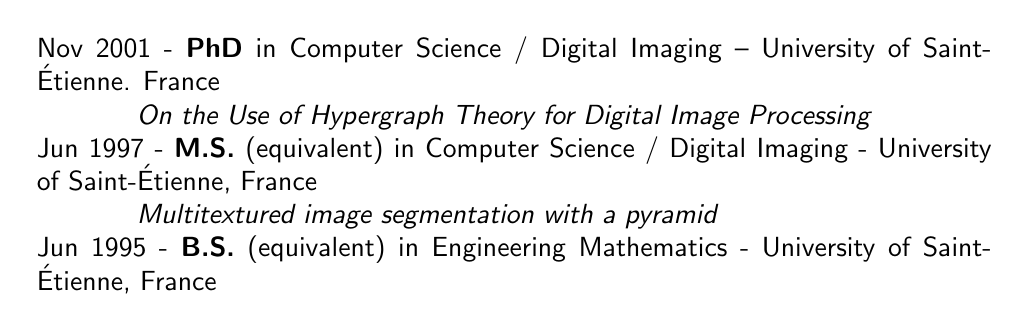
\begin{tikzpicture}
  \node (origin) [rectangle, minimum width=\linewidth,
  anchor=south west] {
    \begin{minipage}{1.0\linewidth}
      Nov 2001 - \textbf{PhD} in Computer Science / Digital Imaging –
      University of Saint-Étienne. France

      \hspace*{.5in}\emph{On the Use of Hypergraph Theory for Digital Image Processing}

      Jun 1997 - \textbf{M.S.} (equivalent) in Computer Science /
      Digital Imaging - University of Saint-Étienne, France

      \hspace*{.5in}\emph{Multitextured image segmentation with a pyramid}

      Jun 1995 - \textbf{B.S.} (equivalent) in Engineering Mathematics -
      University of Saint-Étienne, France
    \end{minipage}
  };
\end{tikzpicture}

\mynewsection{Miscellaneous}{\faBookmark}

Languages: French (native), German (Written and oral comprehension)

Google scholar link: \url{https://scholar.google.com/citations?user=Dw3bjDYAAAAJ&hl=en}

% Scuba diving: Hawai`i, Australia, Palau

\end{document}
